\documentclass[10pt,a4paper,titlepage]{article}

\usepackage[utf8]{inputenc}
\usepackage[T1]{fontenc}

\usepackage[pdftex]{graphicx}
\usepackage[ngerman]{babel}
\usepackage[margin=2.5cm]{geometry}
\usepackage{xcolor}
\usepackage{colortbl}
\usepackage{fancyhdr}

\usepackage{amsmath}
\usepackage{amsfonts}
\usepackage{amssymb}
\usepackage{esint}

\pagestyle{fancy}
\fancyhf{}
\fancyhead[R]{Seite \thepage}
\fancyhead[L]{Physik Formelsammlung}
\fancyhead[C]{Nicolas Trüssel}

\newcommand{\fracsize}{\rule[-2ex]{0pt}{5ex}}
\newcolumntype{C}[1]{>{\fracsize\centering\arraybackslash}m{#1}<{}}

% Custom commands
\newcommand{\unitof}[1]{\left[ \mathrm{#1} \right]}
\newcommand{\abs}[1]{\left| #1 \right|}
\newcommand{\norm}[1]{\left\Vert #1 \right\Vert}
\newcommand{\diff}[2]{\frac{\mathrm d #1}{\mathrm d #2}}
\newcommand{\multidiff}[3]{\frac{\mathrm d^#3 #1}{\mathrm d #2^#3}}
\newcommand{\pdiff}[2]{\frac{\partial #1}{\partial #2}}
\newcommand{\e}[1]{\vec{e}_{#1}}
\renewcommand{\d}{\,\mathrm{d}}
\renewcommand{\vec}[1]{\mathbf{#1}}

\numberwithin{equation}{section}

\begin{document}

\title{Physik Formelsammlung}
\author{Nicolas Trüssel}
%\maketitle

% !TeX root = ../Formelsammlung.tex
\section{Konstanten}
\begin{tabular}{l l l l l}
Gravitationskonstante 									& $G$ 	& 6,673 			& $ \cdot 10 ^ {-11} $ 	& $N m^2kg^{-2}$ \\
Lichtgeschwindigkeit im Vakuum 							& $c$ 	& 299 792 458 	& 						& $ ms^{-1} $ \\
Normwert der Fallbeschleunigung 							& $g$ 	& 9,80665		& 						& $ ms^{-1} $ \\\hline
Mittlerer Erdradius										& $r_E$ 	& 6,3713			& $ \cdot 10 ^ {6} $		& $ m $ \\
Erdmasse													& $m_E$ 	& 5,979			& $ \cdot 10 ^ {24} $	& $ kg $ \\
Fluchtgeschwindigkeit der Erde							& $v_E$	& 1,119			& $ \cdot 10 ^ {4} $ 	& $ ms^{-1} $ \\\hline\hline
Ausbreitungsgeschwindigkeit in Luft ($0 ^\circ$C)			&		& 331			&						& $ ms^{-1} $ \\
Ausbreitungsgeschwindigkeit in Luft ($20 ^\circ$C)		&		& 343			&						& $ ms^{-1} $ \\
Ausbreitungsgeschwindigkeit in He ($20 ^\circ$C)			&		& 965			&						& $ ms^{-1} $ \\
Ausbreitungsgeschwindigkeit in H ($20 ^\circ$C)			&		& 1284			&						& $ ms^{-1} $ \\\hline
Ausbreitungsgeschwindigkeit in Wassser ($0^\circ$C)		&		& 1402			&						& $ ms^{-1} $ \\
Ausbreitungsgeschwindigkeit in Wassser ($20^\circ$C)		&		& 1482			&						& $ ms^{-1} $ \\
Ausbreitungsgeschwindigkeit in Seewassser ($20^\circ$C)	&		& 1522			&						& $ ms^{-1} $ \\\hline
Ausbreitungsgeschwindigkeit in Aluminium 				&		& 6420			&						& $ ms^{-1} $ \\
Ausbreitungsgeschwindigkeit in Stahl		 				&		& 5941			&						& $ ms^{-1} $ \\
Ausbreitungsgeschwindigkeit in Granit	 				&		& 6000			&						& $ ms^{-1} $ \\\hline
Elastizitätsmodul von Aluminium							&		& 100			& $ \cdot 10 ^ {9} $		& $ Nm^{-2} $ \\
Elastizitätsmodul von Stahl								&		& 200			& $ \cdot 10 ^ {9} $		& $ Nm^{-2} $ \\
Elastizitätsmodul von Granit								&		& 200			& $ \cdot 10 ^ {9} $		& $ Nm^{-2} $ \\\hline\hline
Elementarladung											& $e$	& 1,602177		& $ \cdot 10 ^ {-19}$	& $ C $		\\
Avogadrozahl												& $N_A$ 	& 6,02			& $ \cdot 10 ^ {23}$		& $ mol^{-1}$ \\
\end{tabular}
% !TeX root = ../Formelsammlung.tex
\section{Einheiten}
\begin{align*}
\unitof{U} &= \mathrm{V} = \mathrm{\frac{W}{A}} = \mathrm{\frac{J}{C}}\\
\unitof{B} &= \mathrm{T} = \mathrm{\frac{kg}{As^2}} = \mathrm{\frac{Vs}{m^2}}\\[1em]
\unitof{\omega} &= \mathrm{\frac{rad}{s}}
\end{align*}
% !TeX root = ../Formelsammlung.tex
\section{Zehnerpotenzen}
\begin{center}
\begin{tabular}{|C{2.5cm}|C{2.5cm}|C{2.5cm}|}
\hline
\rowcolor[gray]{0.9}
Name		&	Symbol	&	Zehnerpotenz 	\tabularnewline\hline
Yokto	&	y		&	$10^{-24}$		\tabularnewline\hline
Zepto	&	z		&	$10^{-21}$		\tabularnewline\hline
Atto		&	a		&	$10^{-18}$		\tabularnewline\hline
Femto	&	f		&	$10^{-15}$		\tabularnewline\hline
Piko		&	p		&	$10^{-12}$		\tabularnewline\hline
Nano		&	n		&	$10^{-9}$		\tabularnewline\hline
Mikro	&	$\mu$	&	$10^{-6}$		\tabularnewline\hline
Milli	&	m		&	$10^{-3}$		\tabularnewline\hline
Zenti	&	c		&	$10^{-2}$		\tabularnewline\hline
Dezi		&	d		&	$10^{-1}$		\tabularnewline\hline\hline
Deka		&	da		&	$10^1$			\tabularnewline\hline
Hekto	&	h		&	$10^2$			\tabularnewline\hline
Kilo		&	k		&	$10^3$			\tabularnewline\hline
Mega		&	M		&	$10^6$			\tabularnewline\hline
Giga		&	G		&	$10^9$			\tabularnewline\hline
Tera		&	T		&	$10^{12}$		\tabularnewline\hline
Peta		&	P		&	$10^{15}$		\tabularnewline\hline
Exa		&	E		&	$10^{18}$		\tabularnewline\hline
Zetta	&	Z		&	$10^{21}$		\tabularnewline\hline
Yotta	&	Y		&	$10^{24}$		\tabularnewline\hline
\end{tabular}
\end{center}
% !TeX root = ../Formelsammlung.tex
\section{Grundlagen}
\subsection{Koordinatiensysteme}
\begin{equation}
\begin{pmatrix} x \\ y \\ z\end{pmatrix} = 
\begin{pmatrix}r \sin\vartheta \cos\varphi \\ r \sin\vartheta \sin\varphi \\ r \cos\vartheta \end{pmatrix} =
\begin{pmatrix}\rho \cos\varphi \\ \rho \sin\varphi \\ z \end{pmatrix}
\end{equation}
\begin{equation}
\begin{pmatrix} r \\ \varphi \\ \vartheta \end{pmatrix} =
\begin{pmatrix} \sqrt{x^2 + y^2 + z^2}  \\ \arctan\left(y/x\right) \\ \arctan\left(z/r\right) \end{pmatrix}
,\quad
\begin{pmatrix} \rho \\ \varphi \\ z \end{pmatrix} =
\begin{pmatrix} \sqrt{x^2 + y^2} \\ \arctan\left(y/x\right) \\ z \end{pmatrix}
\end{equation}

\subsection{Das Vektorprodukt}
\begin{center}
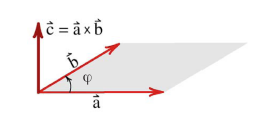
\includegraphics[scale=0.4]{./images/VectorProduct.png}
\end{center}
\begin{equation}
\vec{c} = \vec{a} \times \vec{b} \quad\Rightarrow\quad \vec{\abs{c}} = \vec{\abs{a}}\vec{\abs{b}}\sin\varphi
\end{equation}

\subsection{Ableitungen von Vektoren}
\begin{equation}
\diff{}{t}\left(c \cdot \vec{a}\right) =  \left( \diff{c}{t} \cdot \vec{a} \right) + \left( c \cdot \diff{\vec{a}}{t} \right) 
\end{equation}
\begin{equation}
\diff{}{t}\left(\vec{a} \cdot \vec{b}\right) =  \left( \diff{\vec{a}}{t} \cdot \vec{b} \right) + \left( \vec{a} \cdot \diff{\vec{b}}{t} \right) 
\end{equation}
\begin{equation}
\diff{}{t}\left(\vec{a} \times \vec{b}\right) =  \left( \diff{\vec{a}}{t} \times \vec{b} \right) + \left( \vec{a} \times \diff{\vec{b}}{t} \right) 
\end{equation}

\subsection{Lokales Systeme}
\subsubsection{Kugelkoordinaten}
Die lokalen Einheitsvektoren sind $\e{r}, \e{\vartheta}, \e{\varphi} $ wobei gilt:
\begin{itemize}
\item $\e{r}$ ist radial.
\item $\e{\vartheta}$ zeigt in die Richtung in welche sich der Punkt bewegt wenn $\vartheta$ zunimmt.
\item $\e{\varphi}$ zeigt in die Richtung in welche sich der Punkt bewegt wenn $\varphi$ zunimmt.
\end{itemize}
\begin{center}
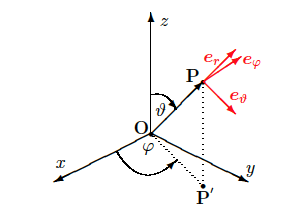
\includegraphics[scale=0.5]{./images/Kugeleinheitsvektoren.png}
\end{center}
\begin{equation}
\begin{pmatrix}
\e{r} \\ \e{\vartheta} \\ \e{\varphi}
\end{pmatrix} =
\begin{pmatrix}
\sin\vartheta\cos\varphi 	& \sin\vartheta\sin\varphi 	& \cos\vartheta \\
\cos\vartheta\cos\varphi 	& \cos\vartheta\sin\varphi 	& -\sin\vartheta \\
-\sin\varphi				 	& \cos\varphi			 	& 0
\end{pmatrix}
\begin{pmatrix}
\e{x} \\
\e{y} \\
\e{z}
\end{pmatrix}
\end{equation}
% !TeX root = ../Formelsammlung.tex
\section{Kinematik}
\subsection{Weg, Geschwindigkeit, Beschleunigung -- Eindimensional}
\begin{equation}
v(t) = \diff{}{t}x(t), \quad a(t) = \diff{v}{t} = \multidiff{x}{t}{2}
\end{equation}
\begin{equation}
x(t) = \int_{t_0}^t\!v(t^\prime)\d t^\prime + x_0, \quad v(t) = \int_{t_0}^t\!a(t^\prime)\d t^\prime + v_0
\end{equation}

\subsection{Weg, Geschwindigkeit, Beschleunigung -- Zweidimensional}
\subsubsection{Kartesische Koordinaten}
\begin{equation}
\vec{r}(t) = x(t)\cdot \e{x} + y(t) \cdot \e{y}
\end{equation}
\begin{equation}
\vec{v}(t) = v_x(t)\cdot \e{x} + v_y(t) \cdot \e{y} = \diff{x}{t} \cdot \e{x} + \diff{y}{t} \cdot \e{y}
\end{equation}
\begin{equation}
\vec{a}(t) = a_x(t)\cdot \e{x} + a_y(t) \cdot \e{y} = \diff{v_x}{t} \cdot \e{x} + \diff{v_y}{t} \cdot \e{y} = \multidiff{x}{t}{2} \cdot \e{x} + \multidiff{y}{t}{2} \cdot \e{y}
\end{equation}

\subsubsection{Kugelkoordinaten}
\begin{equation}
\vec{r}(t) = r(t)\cdot \e{r}
\end{equation}
\begin{equation}
\vec{v}(t) = \diff{r}{t} \cdot \e{r} + r \cdot \diff{\e{r}}{t} = \diff{r}{t} \cdot \e{r} + r \cdot \diff{\varphi}{t} \cdot \e{\varphi} \quad\Rightarrow\quad  v_\varphi = r \cdot \diff{\varphi}{t} 
\end{equation}
\begin{equation}
\vec{a}(t) = \left\{ \multidiff{r}{t}{2} - r \left( \diff{\varphi}{t} \right)^2 \right\} \cdot \e{r} + \left\{ 2 \diff{r}{t}\diff{\varphi}{t} + \multidiff{\varphi}{t}{2} \right\} \cdot \e{\varphi}
\end{equation}

\subsection{Gleichförmige Kreisbewegung}
\begin{equation}
\vec{r}(t) = r \cos\varphi (t) \, \e{x} + r \sin \varphi (t) \, \e{y},\quad r \text{ konstant }
\end{equation}
\begin{equation}
\varphi(t) = \omega t, \quad \omega = \dfrac{2\pi}{T} 
\end{equation}
$\omega$ wird Winkelgeschwindigkeit genannt, Einheit: $\mathrm{rad} / s$ oder $ {}^{\circ} / s$
\begin{equation}
\vec{v}(t) = r \omega \e{\varphi} = - r \omega \sin \omega t \, \e{x} + r \omega \cos \omega t \, \e{y} , \quad \vec{\abs{v}} = r \omega
\end{equation}
\begin{equation}
\vec{a}(t) = - \omega ^2 \vec{r}, \quad \vec{\abs{a}} = \omega ^2 r = \dfrac{v^2}{r}
\end{equation}
% !TeX root = ../Formelsammlung.tex
\section{Dynamik}
\subsection{Der lineare Impuls}
\begin{equation}
\vec{p} = m \vec{v}
\end{equation}
\subsection{Newtons Gesetze}
\subsubsection{Trägheit}
Für isolierte Systeme gilt:
\begin{equation}
\vec{p}_{tot} = \text{konst.} \Rightarrow \diff{\vec{p}_{tot}}{t} = 0
\end{equation}
Enthält das System nur einen Körper so folgt:
\begin{equation}
\diff{\vec{p}}{t} = \diff{(m \vec{v})}{t} = m \diff{\vec{v}}{t} = 0 \quad\Rightarrow\quad \vec{v}(t) = \text{konst.} \quad\Rightarrow\quad \vec{a}(t) = 0
\end{equation}
D. h. ein isolierter Körper bewegt sich gleichförmig.
\subsubsection{Aktionsprinzip}
\begin{equation}
\vec{F} \equiv \diff{\vec{p}}{t} \quad\Rightarrow\quad \vec{F} = m \vec{a}(t)
\end{equation}
\subsubsection{Aktion = Reaktion}
Wir betrachten ein System mit zwei Körpern A und B:
\begin{gather}
\vec{p}_{tot} = \vec{p}_A + \vec{p}_B = \text{konst.} \quad\Rightarrow\quad
\diff{\vec{p}_{tot}}{t} = \diff{\vec{p}_A}{t} + \diff{\vec{p}_B}{t} = 0 \quad\Rightarrow \notag\\
\vec{F}_A + \vec{F}_B = 0 \quad\Rightarrow\quad
\vec{F}_A = - \vec{F}_B
\end{gather}
\subsection{Raketenantrieb}
Wir definieren folgende Grössen
\begin{itemize}
\item $v(t)$ Geschwindigkeit bezüglich festem Koordinatensystem.
\item $u$ Konstante Ausstossgeschwindigkeit des Gases \textit{relativ zur Rakete}. Es gilt $u > 0$.
\item $M(t)$ Gesamtmasse der Rakete zum Zeitpunkt $t$.
\end{itemize}
Zum Zeitpunkt $t$ hat die Rakete einen Impuls von $p(t) = M(t)v(t)$. Zur Zeit $t^\prime = t + \mathrm{d}t$ hat sie eine Masse von $M(t) - \d m$ und eine Geschwindigkeit von $v(t) + \d v$. Es für den Impuls gilt:
\begin{equation}
\begin{split}
p(t^\prime) &= M(t)v(t) + M(t)\d v - v(t) \d m - \d m \d v + v(t) \d m - u \d m \\
	 &\approx  M(t)v(t) + M(t)\d v - u \d m 
\end{split}
\end{equation}
Aus der Impulserhaltung folgt
\begin{equation}
\begin{split}
p(t^\prime) - p(t)	& \approx M(t)v(t) + M(t)\d v - u \d m - M(t)v(t) \\
					& = M(t)\d v - u \d m \\
					& \equiv 0
\end{split}
\end{equation}
\begin{equation}
M(t) \d v = u \d m \quad\Rightarrow\quad M(t) \diff{v}{t} = u \diff{m}{t}
\end{equation}
\begin{equation}
F = u \diff{m}{t}
\end{equation}
Durch Integration erhalten wir:
\begin{equation}
v = u \ln \left(\dfrac{1}{1 - m/M_0} \right)
\end{equation}
wobei m(t) die Gesamtmasse \textbf{des ausgestossenen Gases} zur Zeit t beschreibt.
\subsection{Harmonische Schwingungen}
\begin{equation}
\begin{aligned}
&x(t) = A \sin \left( \omega t + \delta \right) \\
&v(t) = A \omega \cos \left( \omega t + \delta \right) \\
&a(t) = -A \omega ^2 \sin \left( \omega t + \delta \right) = - \omega ^2 x(t)
\end{aligned} \qquad
T = \dfrac{2 \pi}{\omega}, \quad f = \nu = \dfrac{1}{T}
\end{equation}
\subsubsection{Die Differentialgleichung der harmonischen Bewegung}
\begin{equation}
F(t) = -kx(t), \quad \text{wobei hier} \enspace k = m \omega ^2
\end{equation}
\begin{equation}
\multidiff{x}{t}{2} + \dfrac{k}{m}x = 0
\end{equation}
Setzt man $x(t) = A \sin \left( \omega t + \delta \right)$ als Lösung ein, erhält man
\begin{equation}
\omega = \sqrt{\dfrac{k}{m}} \quad\Rightarrow\quad T = 2\pi\sqrt{\dfrac{m}{k}}
\end{equation}\\
wobei k die Rückstellkraftkonstante (Proportionalitätsfaktor zwischen Verschiebung und Rückstellkraft) ist.
\subsection{Gravitation}
\begin{equation}
\vec{F}_{12} = -\dfrac{G m_1 m_2}{r_{12}^2} \cdot \dfrac{\vec{r}_{12}}{r_{12}}
\end{equation}
\subsection{Drehimpuls und -moment}
Drehimpuls: $$\vec{L} \equiv \vec{r} \times \vec{p} \equiv m \left( \vec{r} \times \vec{v} \right)$$ 
Drehmoment: $$\vec{M} \equiv \vec{r} \times \vec{F} = \diff{\vec{L}}{t}$$ 
Wirkt kein Drehmoment bleibt der Drehimpuls erhalten.
% !TeX root = ../Formelsammlung.tex
\section{Energie und Arbeit}
\subsection{Energie}
\subsubsection{Energieerhaltung}
\begin{align}
\begin{split}
E_{tot} 	&= E_{Masse} + E_{kin} + E_{pot} + E_{chem} + \text{usw.} \\
		&= \text{konst.}
\end{split}
\intertext{aber für die Energie eines Körpers (ohne Reibung)}
E &= E_{kin} + E_{pot} \neq \text{konst.} 
\end{align}
\subsubsection{Geschwindigkeitsparameter}
\begin{equation}
\beta \equiv \dfrac{v}{c} = \frac{pc}{E} = \sqrt{1 - \frac{(mc^2)^2}{E_{tot}^{2}}}
\end{equation}
\subsubsection{Relativistischer Impuls}
\begin{equation}
\vec{p} = \gamma m \vec{v}
\end{equation}
\begin{equation}
\gamma \equiv \dfrac{1}{\displaystyle\sqrt{1 - \beta^2}} \qquad \text{Lorentzfaktor}
\end{equation}
\subsubsection{Masse-Energie Äquivalenz}
\begin{equation}
E = mc^2
\end{equation}
\begin{equation}
E_{tot} = \sqrt{c^2p^2 + m^2c^4}
\end{equation}
\subsubsection{Kinetische Energie}
Relativistisch:
\begin{equation}
E = mc^2 + E_{kin} \wedge E = \gamma mc^2 \quad\Rightarrow\quad E_{kin} = mc^2(\gamma - 1)
\end{equation}
Klassisch
\begin{equation}
E_{kin} = \dfrac{1}{2} m v^2
\end{equation}
\subsubsection{Potentielle Energie}
\begin{equation}
E_{pot} = m g h
\end{equation}
\subsection{Arbeit}
Die Arbeit, die eine Kraft an einem Körper leistet, ist gleich dem Produkt der Komponente der Kraft längs der Verschiebung und der Verschiebung ($\vartheta$ ist der Winkel zwischen Kraft und Richtung).
\begin{equation}
W = F \Delta x \cos \vartheta
\end{equation}
\subsubsection{Arbeit und potentielle Energie}
\begin{equation}
\Delta E_{pot} = -W
\end{equation}
Diese Gleichung gilt allgemein für \textbf{konservative} Kräfte.
\subsubsection{Bewegung in mehr Dimensionen}
Gegeben sei ein Vektorfeld $\vec{F} = \vec{F}(\vec{r})$ und zwei Punkte $\vec{r_1}, \vec{r_2}$. Die geleistete Arbeit entlang einer differentiellen Strecke $\d W$ ist gleich $ \vec{F}(\vec{r}) \cdot \d \vec{r}$
\begin{equation}
W_{12} = \int_{\vec{r_1}}^{\vec{r_2}} \d W = \int_{\vec{r_1}}^{\vec{r_2}} \vec{F}(\vec{r}) \d \vec{r}
\end{equation}
Dieses Integral hängt vom Weg zwischen $\vec{r_1}$ und $\vec{r_2}$ ab!
\subsection{Beziehung zwischen Kraft und potentieller Energie}
\subsubsection{Der Gradient}
\begin{equation}
\nabla \equiv 
\begin{pmatrix}
\pdiff{}{x} \\[0.3em]
\pdiff{}{y} \\[0.3em]
\pdiff{}{z}
\end{pmatrix}
\end{equation}
Es gilt:
\begin{equation}
\d f = \nabla f \d \vec{r}
\end{equation}
\begin{equation}
\vec{F} = -\nabla E_{pot}
\end{equation}
\subsection{Arbeit-Energie-Theorem}
Die Arbeit die an einem Körper zwischen zwei Punkten geleistet wird ist:
\begin{equation}
W_{12} = \int_{r_1}^{r_2} \vec{F} \d \vec{r} = \frac{1}{2}m\vec{v_2}^2 - \frac{1}{2}m \vec{v_1}^2
\end{equation}
\subsubsection{Die Fluchtgeschwindigkeit}
Hier ist die wirkende Kraft die Gravitationskraft. Die Bahnkurve des Körpers hat keinen Einfluss, die Arbeit hängt nur von der radialen Bewegung des Körpers ab. Somit ergibt sich:
\begin{equation}
W_{12} = \frac{1}{2}m\vec{v_2}^2 - \frac{1}{2}m \vec{v_1}^2 = G m_E m \left( \frac{1}{r_2} - \frac{1}{r_1} \right)
\end{equation}
Nun wird abgeschätzt: $v_2 \to 0, r_2 \to \infty$, was zu folgender Gleichung führt:
\begin{equation}
\vec{v_1}^2 = 2 g r_1
\end{equation}
\subsection{Allgmeine potentielle Energie der Gravitationskraft}
\begin{equation}
E_{pot}(r) = - G \frac{m_e m}{r}
\end{equation}
% !TeX root = ../Formelsammlung.tex
\section{Wellen}
\subsection{Die Wellenfunkton}
Eine Welle ist von Ort und Zeitpunkt abhängig:
\begin{equation}
\xi = \xi (x, t)
\end{equation}
wobei Ortsabhängigkeit die Form der Welle und die Zeitabhängigkeit die Ausbreitung der Welle beschreiben. Für die Ausbreitungsgeschwindigkeit $v$ kann man auch folgende Gleichung formulieren ($+$ für Ausbreitung in negative x-Richtung, $-$ für Ausbreitung in positive x-Richtung): 
\begin{equation}
\xi (x, t) = \xi(t \pm vt)
\end{equation}
\subsection{Die harmonische Welle}
\begin{equation}
\xi (x, t) = \xi _0 \sin \left( k \left( x \pm vt \right) \right)
\end{equation}
wobei $k$ die Wellenzahl und $\xi _0$ die Amplitude ist. Weitere Beziehungen sind:
\begin{equation}
k = \dfrac{2 \pi}{\lambda}, \qquad f = \nu = \dfrac{\omega}{2 \pi} \quad\Leftrightarrow\quad \omega = 2 \pi \nu
\end{equation}
Somit kann man die Wellengleichung auch so formulieren:
\begin{equation}
\xi (x, t) = \xi _0 \sin \left( k x \pm \omega t  \right), \qquad \text{wobei} \enspace v = \dfrac{\omega}{k} = \nu \lambda
\end{equation}
\subsection{Die Wellengleichung}
\begin{equation}
\pdiff{^2 \xi}{t^2} - v^2 \pdiff{^2 \xi}{x^2} = 0
\end{equation}
Lösung:
\begin{equation}
\xi (x, t) = f(x -vt) - g(x + vt)
\end{equation}
\subsection{Seilwellen}
\begin{equation}
\text{Längendichte:} \quad \rho = \frac{M}{L} \quad\Rightarrow\quad \d m = \rho \d x
\end{equation}
\begin{equation}
v = \pm \sqrt{\frac{S}{\rho}}
\end{equation}
\subsection{Wellen in Festkörpern}
Die relative Längendehnung eines Stabes ist 
\begin{equation}
\varepsilon = \dfrac{\ell}{\Delta \ell} 
\end{equation}
Das Hookesche Gesetz lautet darauf angepasst:
\begin{equation}
F = Y \! A \varepsilon, \quad \text{wobei } Y \text{ das Elastizitätsmodul bezeichnet.}
\end{equation}
\subsubsection{Longitudinale elastische Welle}
Für die Ausbreitungsgeschwindigkeit $v$ der longitudinalen elastischen Welle in einem Festkörper gilt:
\begin{equation}
v = \sqrt{\dfrac{Y}{\rho}} 
\end{equation}
wobei $\rho$ hier die Volumendichte bezeichnet und $Y$ das oben erwähnte Elastizitätsmodul ist.
\subsection{Superposition harmonischer Wellen}
\begin{equation}
\xi (x_1, \Delta x, t) = \underbrace{2A \cos \left\{ \dfrac{1}{2} \left( \delta + k \Delta x \right) \right\}}_{\text{Amplitude}} \underbrace{ \sin \left\{ kx_1 - \omega t + \dfrac{1}{2} \left( \delta + k \Delta x \right) \right\}}_{\text{harmonische Welle}}
\end{equation}
% !TeX root = ../Formelsammlung.tex
\section{Relativsysteme, Inertialsysteme und Relativitätstheorie}
\subsection{Transformation zwischen Bezugssystemen}
\begin{center}
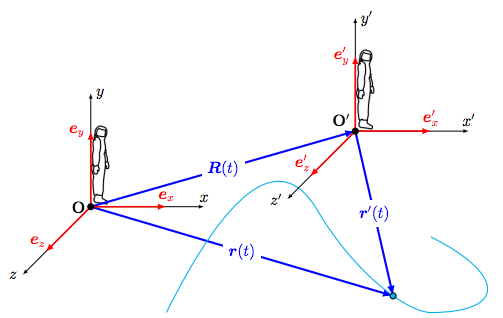
\includegraphics[scale=0.5]{./images/Bezugssysteme.png}
\end{center}
\begin{equation}
\begin{cases}
\vec{r} (t) = \vec{R} (t) + \vec{r^\prime} (t^\prime) \\
t = t^\prime
\end{cases}
\qquad
\begin{cases}
\vec{r^\prime} (t^\prime) = - \vec{R} (t) + \vec{r} (t) \\
t^\prime = t
\end{cases}
\end{equation}
\begin{equation}
\vec{v}(t) = \diff{\vec{R}(t)}{t} + \vec{v^\prime} (t)
\end{equation}
\begin{equation}
\vec{a}(t) = \multidiff{\vec{R}(t)}{t}{2} + \vec{a^\prime} (t)
\end{equation}
\subsection{Inertialsysteme}
Ein Bezugssystem in dem die Newtonschen Gesetze gelten wird Inertialsystem genannt. Das heisst, dass sich verschiedene Inertialsysteme relativ zueinander mit konstanter Geschwindigkeit bewegen.
\subsection{Beschleunigte Systeme, Scheinkräfte}
Wird ein Körper in einem Inertialsystem beschleunigt so gilt $\vec{F} = m \vec{a}$. In einem beschleunigten Bezugssystem gilt jedoch:
\begin{equation}
\vec{F} \neq m \vec{a^\prime} = m \left( \vec{a} - \multidiff{\vec{R}(t)}{t}{2} \right)
\end{equation}
aber:
\begin{equation}
\vec{F^\prime} = m \vec{a^\prime} = m \left( \vec{a} - \multidiff{\vec{R}(t)}{t}{2} \right) \quad\Rightarrow\quad \vec{F^\prime} = \vec{F} + \underbrace{\multidiff{\vec{R}(t)}{t}{2}}_{\text{Scheinkraft}}
\end{equation}
\subsubsection{Rotierendes Bezugssytem}
Annahme: $\omega$ konstant. 
\paragraph{Die Zentrifugalkraft}
\begin{equation}
\vec{F}_{ZP} = m \left(r^\prime \omega ^2 \right) \e{r}
\end{equation}
\paragraph{Die Corioliskraft}
\begin{equation}
\vec{F}_{C} = m \left(2 v^\prime \omega \right) \e{\varphi}
\end{equation}
\subsection{Galileitransformation}
Betrachtet werden 2 Bezugssysteme die sich relativ zueinander mit konstanter Geschwindigkeit $\vec{V}$ bewegen.
\begin{align}
\vec{r^\prime}(t) &= \vec{r} (t) - \vec{V} t \\
\vec{v^\prime} &= \vec{v} - \vec{V} \\
\vec{a^\prime}(t) &= \vec{a}(t)
\end{align}
\subsubsection{Raumzeit}
\begin{equation}
x^\mu \equiv 
\begin{pmatrix}
ct & x & y & z
\end{pmatrix}
\end{equation}
Die Galileitransformation kann nun so geschrieben werden:
\begin{equation}
\underbrace{
\begin{pmatrix}
ct^\prime \\
x^\prime \\
y^\prime \\
z^\prime
\end{pmatrix}
}_{x^{\prime \mu}}
= 
\underbrace{
\begin{pmatrix}
1 		& 0 & 0 & 0 \\
-\beta 	& 1 & 0 & 0 \\
0		& 0 & 1 & 0 \\
0		& 0 & 0 & 1
\end{pmatrix}
}_{M_G (\beta)}
\underbrace{
\begin{pmatrix}
ct \\
x \\
y \\
z
\end{pmatrix}
}_{x^\mu}
\end{equation}
Die Inverse lautet:
\begin{equation}
\underbrace{
\begin{pmatrix}
ct \\
x \\
y \\
z
\end{pmatrix}
}_{x^\mu}
= 
\underbrace{
\begin{pmatrix}
1 		& 0 & 0 & 0 \\
+\beta 	& 1 & 0 & 0 \\
0		& 0 & 1 & 0 \\
0		& 0 & 0 & 1
\end{pmatrix}
}_{M_G^{-1} (\beta)}
\underbrace{
\begin{pmatrix}
ct^\prime \\
x^\prime \\
y^\prime \\
z^\prime
\end{pmatrix}
}_{x^{\prime \mu}}
\end{equation}
\subsection{Lorentztransformation}
\begin{equation}
\begin{pmatrix}
ct^\prime \\
x^\prime \\
y^\prime \\
z^\prime
\end{pmatrix}
= 
\begin{pmatrix}
\gamma			& -\beta \gamma	& 0 & 0 \\
-\beta \gamma	& \gamma			& 0 & 0 \\
0		& 			0 			& 1 & 0 \\
0		& 			0 			& 0 & 1
\end{pmatrix}
\begin{pmatrix}
ct \\
x \\
y \\
z
\end{pmatrix}
\end{equation}
Für die Inverse gilt wiederum:
\begin{equation}
\begin{pmatrix}
ct \\
x \\
y \\
z
\end{pmatrix}
= 
\begin{pmatrix}
\gamma			& +\beta \gamma	& 0 & 0 \\
+\beta \gamma	& \gamma			& 0 & 0 \\
0		& 			0 			& 1 & 0 \\
0		& 			0 			& 0 & 1
\end{pmatrix}
\begin{pmatrix}
ct^\prime \\
x^\prime \\
y^\prime \\
z^\prime
\end{pmatrix}
\end{equation}
\subsection{Die Raumzeit}
Da bei relativistischem Ansatz:
\begin{equation}
\Delta t \neq \Delta t^\prime \quad\Rightarrow\quad \Delta x \neq \Delta x^\prime \quad\Rightarrow\quad \Delta r \neq \Delta r^\prime
\end{equation}
(Von verschiedenen Beobachteren gemessene Zeitintervalle zwischen zwei Ereignissen sind nicht immer gleich). Das Raumzeit-Intervall $\Delta s$ ist jedoch für alle Beobachter identisch. 
\begin{equation}
\begin{split}
\Delta s ^2 	& \equiv (c \Delta t)^2 - \Delta r ^2 \\
			& = (c \Delta t)^2 - \Delta x ^2 - \Delta y ^2 - \Delta z ^2
\end{split}
\end{equation}
\subsubsection{Zeitdilatation}
Ist $\Delta \tau $ die in einem unbewegten System gemessene Zeitdifferenz zwischen zwei Ereignissen so gilt in einem bewegten System für die Zeitdifferenz $\Delta t$:
\begin{equation}
\Delta t = \gamma \cdot \Delta \tau
\end{equation}
\subsubsection{Längenkontraktion}
Da für bewegte Systeme bezüglich unbewegten die Zeit langsamer vergeht, müssen in einem bewegten System auch die Distanzen bezüglich dem unbewegten System kürzer werden. \\
Beispiel: Eine Raktete fliegt mit einer Gewschwindigkeit für die $\gamma = 10$ gilt zu einem für uns 100 Lichtjahre entferneten Planeten. Da die Rakete sich bewegt vergeht in ihr die Zeit langsamer bezüglich der Erde. Sie kann den Planeten darum in 10 Lichtjahren erreichen (Zeitdilatation). Die Strecke die die Rakete dabei zurücklegt ($\gamma = 10 \Rightarrow v \approx c$) beträgt 10 Lichtjahre. Die Länge ist kontrahiert! \\
Ist die ursprüngliche Länge $\Delta \lambda$ so gilt für die Länge $\Delta x$ in einem bewegten System:
\begin{equation}
\Delta x = \dfrac{\Delta \lambda}{\gamma}
\end{equation}
\subsection{Geschwindigkeitstransformation}
Ein Körper K bewegt sich im Bezugssystem $\mathbf{O^\prime}$ mit einer Geschwindigkeit $\vec{u^\prime}$. $\mathbf{O^\prime}$ bewegt sich bezüglich $\mathbf{O}$ mit der Geschwindigkeit $V$ in x-Richtung. K bewegt sich bezüglich $\mathbf{O}$ mit einer Geschwindigkeit $\vec{u}$:
\begin{align}
u_x &= \cfrac{u_x^\prime + V}{1 + \frac{\beta}{c} u_x^\prime} \\
u_y &= \cfrac{u_y^\prime}{\gamma \left( 1 + \frac{\beta}{c}u_x^\prime \right)} \\
u_z &= \cfrac{u_z^\prime}{\gamma \left( 1 + \frac{\beta}{c}u_x^\prime \right)}
\end{align}
% !TeX root = ../Formelsammlung.tex
\section{Thermodynamik}
\subsection{Druck}
\begin{equation}
p = \frac{F}{A} 
\end{equation}
\begin{equation}
\left[ p \right] = \mathrm{Pa}, \quad 1 \, \mathrm{Pa} = 1 \, \mathrm{N} / \mathrm{m^2}, \quad 1 \, \mathrm{bar} = 10^5 \, \mathrm{Pa}, \quad 1 \, \mathrm{atm} = 1,01325 \cdot 10^5 \, \mathrm{Pa}
\end{equation}
\subsection{Gesetz von Gay-Lussac}
\begin{equation}
V = C_1 \cdot T, \quad \text{bei konstantem Druck}, \quad \left( V \propto T \right)
\end{equation}
\subsection{Gesetz von Boyle und Mariotte}
\begin{equation}
p = C_2 \cdot T, \quad \text{bei konstantem Volumen}, \quad \left( p \propto T \right)
\end{equation}
\subsection{Zustandsgleichung des idealen Gases}
\begin{equation}
p \cdot V = n \cdot R \cdot T = N \cdot k \cdot T
\end{equation}
$p$ = Druck, $V$ = Volumen $n$ = Anzahl Mole, $N$ = Anzahl Moleküle, $T$ = absolute Temperatur
\begin{align}
k &= 1,381 \cdot 10^{-23} \mathrm{J / K} \qquad \text{(Boltzmann-Konstante)} \\ 
R &= N_Ak = 8,314 \frac{\mathrm{J}}{\mathrm{mol \cdot K}}
\end{align}
\subsection{Die Standardbedingungen}
\begin{align}
T &= 0^\circ C = 273,15 \text{ K} \\
p &= 1 \text{ atm}
\end{align}
\subsection{Wärmekapazität}
Die Wärmekapazität eines \textbf{Körpers} (als ganzes) ist definiert als
\begin{equation}
C = \frac{\Delta Q}{\Delta T}
\end{equation}
Die \textbf{speifische} Wärmekapazität ist 
\begin{equation}
c = \frac{\Delta Q}{m \Delta T}
\end{equation}
Die \textbf{molare} Wärmekapazität ist 
\begin{equation}
c = \frac{\Delta Q}{n \Delta T}
\end{equation}
Für die Erwärmung eines Körpers von $T_a$ auf $T_e$ wird die Wärmemenge (Energie) $Q$ benötigt:
\begin{equation}
Q = \int \d Q = \int \limits_{T_a}^{T_b} C \left( T \right) \d T
\end{equation}
Für kleine $\Delta T$ gilt
\begin{equation}
Q = C \cdot \Delta T
\end{equation}
\subsubsection{Wärmekapazität des idealen (einatomigen) Gases}
\begin{equation}
C = \frac{3}{2}Nk
\end{equation}
Für die molare Wärmekapazität gilt
\begin{equation}
c = \frac{3}{2}N_Ak = \frac{3}{2} R \approx 12,5 \frac{\mathrm{J}}{\mathrm{mol \cdot K}}
\end{equation}
\subsubsection{Wärmekapazität eines Festkörpers, Dulong-Petit}
Die spezifischen Wärmekapazitäten von Festkörpern variieren stark, die molaren Wärmekapazitäten sind bis auf einige Ausnahmen sehr ähnlich:
\begin{equation}
c \approx 25 \frac{\mathrm{J}}{\mathrm{mol \cdot K}}
\end{equation}
\subsection{Latente Wärme}
\begin{equation}
Q = m \cdot L, \quad \text{wobei L die spezifische latente Wärme und m die Masse ist}
\end{equation}
\subsection{Wärmestrahlung}
\subsubsection{Stefan-Bolzmannsches Gesetz}
Die (über alle Wellenlängen aufsummierte, auf der Fläche normierte und nach vorne abgestrahlte) Wärmestrahlung realer Körper ist
\begin{equation}
S \left( T \right) = \varepsilon \sigma T^4
\end{equation}
Dabei ist $\varepsilon \leq 1$ eine Zahl, die den Emissionsgrad des Körpers bezeichnet (oft temperaturabhängig, $\varepsilon = 1$ für schwarze Stahler) und $\sigma$ ist die Stefan-Bolzmann-Konstante:
\begin{equation}
\sigma = 5,670 \cdot 10^{-8} \frac{\mathrm{W}}{\mathrm{m^2 \cdot K^4}}
\end{equation}
Für einen Körper mit Temperatur $T$ bei einer Umgebungstemperatur $T_0$ gilt:
\begin{equation}
S_\mathrm{netto} = S_\mathrm{emmitiert} - S_\mathrm{absorbiert} = \varepsilon \sigma T^4 - \varepsilon \sigma {T_0}^4
\end{equation}
\subsubsection{Wiensches Verschiebungsgesetz}
\begin{equation}
\lambda_\mathrm{max} = \frac{2898 \mathrm{\mu m} \cdot K}{T}
\end{equation}
Wobei $\lambda_\mathrm{max}$ das Maximum der Spektralverteilungsfunktion $S \left( \lambda, T \right)$ ist (siehe unten).
\subsubsection{Spektralverteilungsfunkton}
Gesetz von Rayleigh-Jeans (Historisch und falsch!!):
\begin{equation}
S \left( \lambda, T \right) = \frac{2 \pi c}{\lambda^4}kT
\end{equation}
$k$ ist die Boltzmann-Konstante, $c$ die Lichtgeschwindigkeit \\[1em]
Gesetz von Plank:
\begin{equation}
S \left( \lambda, T \right) = \frac{2 \pi c^2 h}{\lambda^5} \frac{1}{e^{hc/\left(\lambda k T \right)} - 1}
\end{equation}
$k$ bezeichnet wiederum die Boltzmann-Konstante, $h$ ist die Planksche Konstante
\begin{equation}
h \approx 6,626 \cdot 10^{-34} \,\mathrm{J \cdot s}
\end{equation}
\subsection{Innere Energie}
Die innere Energie $U$ eines Körpers kann sowohl durch Wärmezufuhr als auch durch Leistung mechanischer Arbeit verändert werden. Es gilt:
\begin{equation}
\d U = \d Q + \d W
\end{equation}
\subsection{Mechanische Arbeit eines expandierenden Gases}
Ausgangszustand: Ein Gas mit Druck $p$ befindet sich in einem Behälter, der durch einen reibungsfreien Kolben verschlossen wird. Die vom Gas geleistete Arbeit bei einer Expansion (unabhängig von der Art der Expansion) um $\d V = A \d x$ ist:
\begin{equation}
\d W = -F \d x = - p A  \d x = - p \d V
\end{equation}
\subsection{Thermische Prozesse des idealen Gases}
Allgemein gilt:
\begin{equation}
W = \int\limits_{V_a}^{V_e} \d W = - \int\limits_{V_a}^{V_e}p \d V
\end{equation}
\subsubsection{Isobare Zustandsänderung}
\begin{equation}
W = - p \int\limits_{V_a}^{V_e} \d V = -p \left( V_e - V_e \right)
\end{equation}
\subsubsection{Isotherme Zustandsänderung}
Hier gilt: $$pV = konst.$$
Um die Temperatur des Gases bei der Expansion konstant zu halten, muss Energie zugeführt werden. Da $T$ konstant und die innere Energie $U$ eines idealen Gases nur von $T$ abhängt gilt:
\begin{equation}
\d U = \d Q + \d W = 0 \quad\Rightarrow\quad \d Q = - \d W
\end{equation}
Daraus folgt:
\begin{equation}
Q = - W = - \int\d W = \int\limits_{V_1}^{V_2}p \d V \,\overset{pV=nRT}{=}\, nRT \int\limits_{V_1}^{V_2}\frac{1}{V} \d V = nRT \ln\left(\frac{V_2}{V_1} \right)
\end{equation}
\subsubsection{Adiabatische Expansion}
Bei der adiabatischen Expansion wird keine Wärme ausgetauscht ($\d Q = 0$)
\begin{equation}
\d U - \d W = 0 \quad\Rightarrow\quad C \d T = - \frac{nRT}{V}\d V \quad\Rightarrow\quad \frac{\d T}{T} = - \frac{nR}{C}\frac{\d V}{V}
\end{equation}
\begin{equation}
\gamma \equiv 1 + \frac{nR}{C} \quad\Leftrightarrow\quad \gamma - 1 = \frac{nR}{C}
\end{equation}
\begin{equation}
\int \frac{1}{T}\d T = - \left(\gamma - 1\right) \int\frac{1}{V} \d V \quad\Rightarrow\quad \ln T + \left( \gamma - 1 \right) \ln V = konst.
\end{equation}
Daraus folgt:
\begin{equation}
TV^{\gamma - 1} = konst. \quad\wedge\quad \frac{pV}{nRT}V^{\gamma - 1} = konst. \Rightarrow pV^\gamma = konst.
\end{equation}
Arbeit:
\begin{equation}
\Delta W = \Delta U = c \cdot \Delta T, \quad \gamma = 1 + \frac{nR}{c} \quad \text{umformen und fertig.}
\end{equation}
\subsection{Wirkungsgrad}
Sei $Q_W$ die in warmen Reservoir aufgenommene Wärme, $Q_K$ die im kalten Reservoir abgegebene Wärme und $W = Q_W - Q_K$ die verrichtete Arbeit. Dann gilt für den Wirkungsgrad einer Wärmekraftmaschine:
\begin{equation}
\varepsilon = \frac{\abs{W}}{\abs{Q_W}} = 1 - \frac{\abs{Q_K}}{\abs{Q_W}}
\end{equation}
Im Falle einer carnotschen Wärmekraftmaschine (besser gehts nicht) gilt:
\begin{equation}
\varepsilon = 1 - \frac{T_3}{T_1}
\end{equation}
wobei $T_1$ die Temeperatur des warmen Reservoirs und $T_2$ die Temperatur des kalten Reservoirs ist.
% !TeX root = ../Formelsammlung.tex
\section{Elektromagnetismus}
\subsection{Coulombsches Gesetz}
\begin{equation}
F_c = \frac{1}{4\pi\varepsilon_0}\frac{q_1 q_2}{r^2}
\end{equation}
\begin{equation}
\varepsilon_0 \equiv \frac{10^7}{4\pi c^2}\,\frac{\mathrm{C^2}}{\mathrm{N \cdot m^2}}
\end{equation}
\begin{equation}
e = 1,60217\cdot 10^{-19} \,\mathrm{C}
\end{equation}
\subsection{Elektrisches Feld}
Im Mittelpunkt des Koordinatensystemes befindet sich eine Punktladung $Q$. Das elektrische Feld ist:
\begin{equation}
\vec{E}\left(\vec{r}\right) \equiv \frac{\vec{F\left(\vec{r}\right)}}{q} = \frac{1}{4\pi\varepsilon_0}\frac{Q}{r^2}\frac{\vec{r}}{r}
\end{equation}
\subsection{Elektrische potentielle Energie}
\begin{equation}
E_{pot}^e\left(\vec{r}\right) = \frac{1}{4\pi\varepsilon_0}\frac{q_1 q_2}{r}
\end{equation}
\subsection{Elektrisches Potential}
\begin{equation}
V\left(\vec{r}\right) = \frac{E_{pot}^e\left(\vec{r}\right)}{q}
\end{equation}
Ist das Potential bekannt, so kann das elektrische Feld so berechnet werden:
\begin{equation}
\vec{E}\left(\vec{r}\right) = - \nabla V\left(\vec{r}\right)
\end{equation}
Die Spannung ist gleich dem Potentialunterschied zwischen 2 Punkten:
\begin{equation}
U = V\left(\vec{r_1}\right) - V\left(\vec{r_2}\right) = \int\limits_{r_1}^{r_2}\vec{E}\cdot \d \vec{r}
\end{equation}
\subsection{Elektrische Ladung in elektrischen und magnetischen Feldern}
\subsection{Kraft auf einen elektrischen Strom}
Die Kraft auf einen Leiter mit Querschnittsfläche $A$ und Länge $L$ in einem Magnetfeld $\vec{B}$ ist:
\begin{equation}
\vec{F} = L\vec{I} \times \vec{B}, \quad\text{für differentielle Elemente des Stromes: } \d\vec{F} = L \d\vec{I} \times \vec{B} = I \d\vec{L} \times \vec{B}
\end{equation}
\subsubsection{Lorentz-Kraft}
Sei $\vec{E}$ das elektrische und $\vec{B}$ das magnetische Feld.
\begin{equation}
\vec{F} = \vec{F_E} + \vec{F_B} = q \left( \vec{E} + \vec{v} \times \vec{B} \right)
\end{equation}
\subsubsection{Bewegung einer Punktladung im elektrischen Feld}
\begin{equation}
1 \, \mathrm{eV} = 1,602 \cdot 10^{-19} \mathrm{J}
\end{equation}
Unter Wirkung der elektrischen Kraft erfährt ein Teilchen der Ladung $q$ und Masse $m$ die Beschleunigung (nicht relativistisch!)
\begin{equation}
\vec{a} = \frac{q}{m}\vec{E}
\end{equation}
\subsubsection{Bewegung einer Punktladung im Magnetschen Feld}
Bewegt sich ein Teilchen der Ladung $q$, Masse $m$ und Geschwindigkeit $\vec{v}$ genau senkrecht zu einem homogenen Magnetfeld $\vec{B}$, so beschreibt es eine Kreisbahn mit Radius $r$:
\begin{equation}
r = \frac{m \gamma v}{q B}
\end{equation}
$\gamma$ bezeichnet den Lorentz-Faktor. Die Herleitung geschieht über die Lorentz-Kraft im B-Feld, welche der Zentripetalkraft (relativistisch, also klassische Formel mit $\gamma$ multiplizieren) gleichgesetzt wird.
\subsection{Strom}
\begin{equation}
I\left(t\right) = \frac{\d Q}{\d t}, \qquad\mathrm{Stromdichte}\quad j = \frac{I}{A}
\end{equation}
\subsubsection{Driftgeschwindigkeit}
Seien $e$ die Elementarladung, $n$ die Dichte der beweglichen Elektronen (in $m^{-3}$), $A$ die betrachtete Fläche und $v_D$ die Driftgeschwindigkeit der Elektronen. Es gilt:
\begin{equation}
I = -e n A  v_D
\end{equation}
Andernfalls kann die Driftgeschwindigkeit auch so bestimmt werden: $\tau$ ist die mittlere Zeit zwischen zwei Elektron-Ion Kollisionen, $a$ die Beschleunigung, $\vec{E}$ das elektrische Feld und $\mu = \frac{e\tau}{m}$ die Beweglichkeit der Elektronen.
\begin{equation}
\vec{v}_D = \vec{a} \tau = \frac{-e\vec{E}}{m}\tau = -\mu\vec{E}
\end{equation}
\subsubsection{Das ohmsche Gesetz}
\begin{equation}
U = R I = \left( \frac{L}{\sigma A} \right) I
\end{equation}
wobei $\sigma$ die Leitfähigkeit ist.
\subsection{Kapazität}
\begin{equation}
Q = CV
\end{equation}
Wobei $Q$ die getrennte Ladung, $V$ die Potentialdifferenz und $C$ die Kapazität des Kondensators ist. \\
Die gespeicherte Energie beträgt:
\begin{equation}
E = \frac{Q^2}{2C} = \frac{1}{2}CV^2
\end{equation}
\subsection{Der Fluss}
Der Fluss $\d \Phi$ eines Vektorfeldes $\vec{F}$ durch eine infinitessimale Fläche $\d \vec{A}$ ($\d \vec{A}$ steht senkrecht auf $A$ und hat Betrag des Flächeninhalts) ist:
\begin{equation}
\d \Phi = \vec{F} \cdot \d \vec{A} = \abs{\vec{F}} \abs{d \vec{A}} \cos\vartheta
\end{equation}
$\vartheta$ bezeichnet den Winkel zwischen $\d \vec{A}$ und $\vec{F}$.
Für eine endliche Fläche gilt 
\begin{equation}
\Phi = \iint \vec{F} \d \vec{A}
\end{equation}
Für den aus einem Volumen V austretenden Fluss $\Phi_{tot}$ gilt:
\begin{equation}
\Phi_{tot} = \varoiint\limits_{A = \partial V} \vec{F} \cdot \d \vec{A} = \iiint \left(\vec{\nabla} \cdot \vec{F} \right) \d V
\end{equation}
\subsection{Ladungs- und Stromdichte}
\subsubsection{Ladungsdichte}
\begin{equation}
\rho \left( \vec{r} \right) = \frac{\d q}{\d V} \qquad \text{Raumladungsdichte}
\end{equation}
\begin{equation}
Q = \int \d q = \iiint \rho \left( \vec{r} \right) \d V
\end{equation}
\subsubsection{Stromdichte}
\begin{equation}
I = \iint\limits_A \vec{j} \left( \vec{r} \right) \cdot  \d \vec{A}, \quad \d I = \vec{j} \left( \vec{r} \right) \cdot  \d \vec{A}
\end{equation}
\subsection{Maxwellgleichungen}
\begin{align}
\varepsilon_0 \left( \vec{\nabla} \cdot \vec{E} \right) &= \rho \\
\left( \vec{\nabla} \cdot \vec{B} \right) &= 0 \\
\vec{\nabla} \times \vec{E} &= - \pdiff{\vec{B}}{t} \\
\vec{\nabla} \times \vec{B} &= \mu_0 \vec{j} + \varepsilon_0 \mu_0 \pdiff{\vec{E}}{t}
\end{align}
Dabei sind: 
\begin{align*}
\vec{E} \left(\vec{r}, t \right) &= \text{das elektrische Feld} \\
\vec{B} \left(\vec{r}, t \right) &= \text{das magnetische Feld} \\
\rho \left( \vec{r}, t \right) &= \text{die Ladungsdichte} \\
\vec{j} \left( \vec{r}, t \right) &= \text{die Stromdichte}
\end{align*}
\subsection{Gausstheorem für das elektrische Feld}
Grundlage ist die erste Maxwellgleichung. Daraus folgt mittels dem Theorem von Gauss für alle $\vec{r}$ die ausserhalb des betrachteten Volumens liegen:
\begin{equation}
\varepsilon_0 \varoiint\limits_{A=\partial V}\vec{E}\cdot\d \vec{A} = Q_{eingeschl.} \quad\Rightarrow\quad \abs{\vec{E}\left(\vec{r}\right)} = \frac{Q_{eingeschl.}}{\varepsilon_0 A} 
\end{equation}
\subsection{Divergenz des Magnetfeldes}
Aus der zweiten Maxwellgleichung folgt direkt, dass der Fluss eines Magnetfeldes durch eine geschlossene Oberfläche immer gleich 0 ist.
\subsection{Ampèresches Gesetz}
Ist Folge der dritten Maxwellgleichung für $\pdiff{}{t} = 0$ (zeitunabhängige Vorgänge).
\begin{equation}
\vec{\nabla} \times \vec{B}\left(\vec{r}\right) = \mu_0 \vec{j}\left(\vec{r}\right)
\end{equation}
Mittels Stokes folgt:
\begin{equation}
\oint\limits_{C = \partial A} \vec{B} \d \vec{r} = \mu_0 I
\end{equation}
\subsection{Gesetz von Faraday}
Betrachtet werden die Maxwellgleichungen für einen ladungs- und stromfreien Raum (Vakuum):
\begin{equation}\label{Maxwell:Vakuum}
\begin{cases}
\vec{\nabla} \times \vec{E} &= - \pdiff{\vec{B}}{t} \\
\vec{\nabla} \times \vec{B} &= \varepsilon_0 \mu_0 \pdiff{\vec{E}}{t}
\end{cases}
\end{equation}
Daraus folgt:
\begin{equation}
U_{ind} = \oint\limits_{C = \partial A} \vec{E} \cdot \d \vec{r} = - \diff{\Phi_B}{t} = \diff{}{t}\iint\limits_A \vec{B} \cdot \d A
\end{equation}
\subsection{Elektromagnetische Wellen}
Grundlage bilden die Gleichungen \eqref{Maxwell:Vakuum}. Davon wird je die Rotation gebildet, es ergibt sich:
\begin{equation}
\vec{\nabla}^2\vec{E} = \varepsilon_0 \mu_0 \pdiff{^2\vec{E}}{t^2} \quad\text{und}\quad \vec{\nabla}^2\vec{B} = \varepsilon_0 \mu_0 \pdiff{^2\vec{B}}{t^2}
\end{equation}
Wobei gilt:
\begin{equation}
\vec{\nabla}^2\xi = \pdiff{^2\xi}{x^2} + \pdiff{^2\xi}{y^2} + \pdiff{^2\xi}{z^2} = \varepsilon_0 \mu_0 \pdiff{^2\xi}{t^2} \equiv \frac{1}{v^2}\pdiff{^2\xi}{t^2}
\end{equation}

\end{document}